\section{Abstrahierung}
Nun folgt die Entwicklung eines Operations Orchestrators für die nachfolgenden zwei bis drei beschriebenen Use Cases.

\subsection{Use Cases} 
Die Use Cases (siehe Kapitel \ref{usecases}: Use Cases) sind nach der Nummerierung priorisiert worden. Der UC01 soll auf jeden Fall umgesetzt werden. Der UC02 muss evaluiert werden, ob dies mit der API des DNA Centers im Zusammenspiel mit dem ENCS überhaupt möglich ist. Zu guter Letzt kommt der UC03, welcher nur optional ist und bei genügend verbleibender Zeit implementiert wird.


\subsection{Technologien}
Für das entwickeln des Orchestratortool wird Flask verwendet, welches auf Python basiert. Mit diesem soll eine Web Anwendung entwickelt werden, die auf die vorhandene API des DNA Center und wenn nötig über die API des ENCS Informationen abruft und Konfigurationen vornimmt.

\subsubsection{Python}
Python ist eine objektorientierte Programmiersprache. Die einfache und leicht erlernbare Python-Syntax hebt die Lesbarkeit hervor und reduziert dadurch die Programmwartung. Python unterstützt Module und Pakete, was die Modularität von Programmen und die Wiederverwendung von Code fördert. Der Python-Interpreter und die umfangreiche Standardbibliothek sind in Quell- oder Binärform kostenlos für alle gängigen Plattformen verfügbar und können frei verteilt werden. \cite{python}

\subsubsection{Flask}
Flask ist ein in Python geschriebenes Webframework. Der Fokus von Flask liegt auf Erweiterbarkeit und guter Dokumentation. Die einzigen Abhängigkeiten sind Jinja2, eine Template-Engine, und Werkzeug, eine Bibliothek zum Erstellen von WSGI-Anwendungen. \cite{flask}

\subsubsection{DNA Center Platform}
Cisco hat seit dem Sommer 2018 eine DNA Center Plattform zur Verfügung gestellt, über die nun auf den API Katalog und andere Ressourcen zugegriffen werden kann. So können beispielsweise die Plattform Funktionen auch verwendet werden, um die Bereitstellung und Verwaltung von Netzwerken zu vereinfachen.


So soll das DNA Center nun eine 360 Grad Erweiterbarkeit durch vier verschiedene Plattform Funktionen bereitstellen. Dazu gehören die Intent-based APIs, Process adapters, Domain adapters, sowie SDKs. \cite{dnac-platform}

\begin{figure}[H]
	\centering
	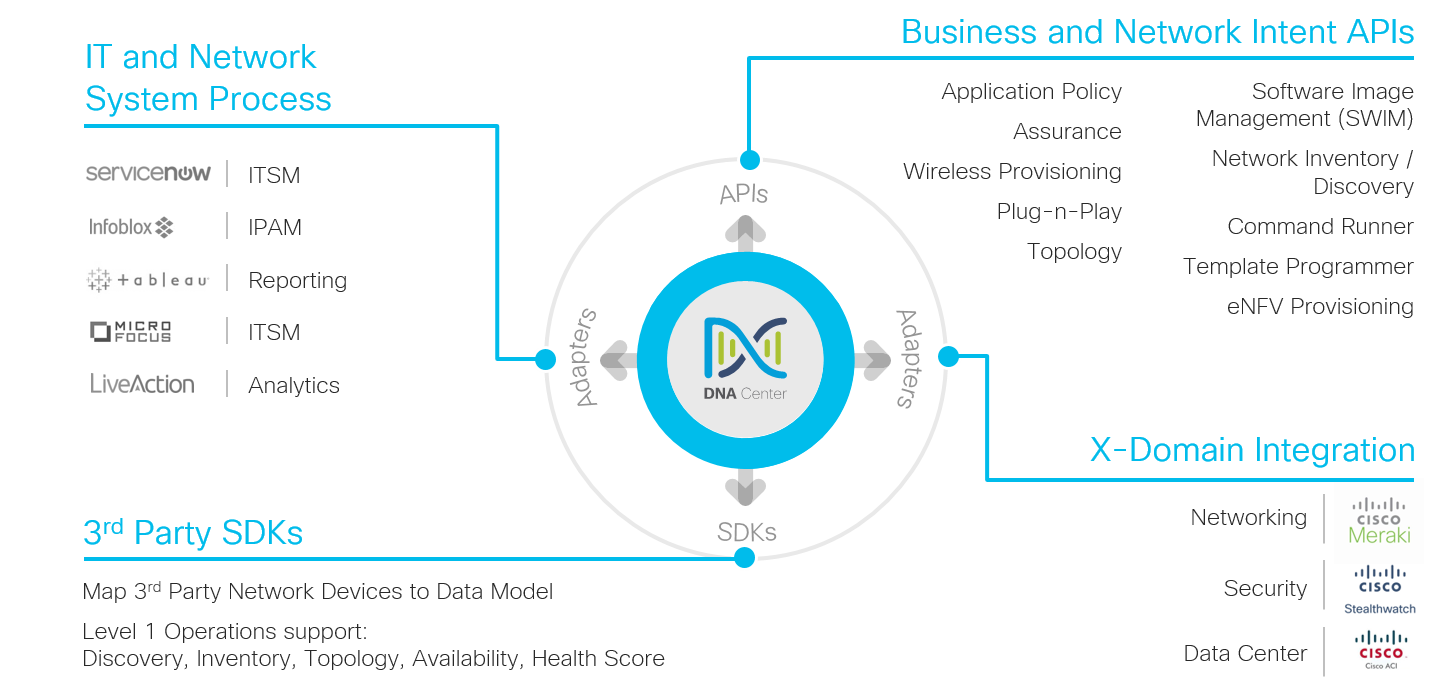
\includegraphics[width=0.8\linewidth]{img/Abstrahierung/dnac-platform}
	\caption{DNA Center Plattform \cite{dnac-platform}}
	\label{fig:DNA Center Plattform}
\end{figure}


\paragraph{DNA Center Intent-API}

Die Intent-API ist eine Northbound REST API, welche bestimmte funktionen des DNA Centers verfügbar macht. Mit der RESTful Intent API des DNA Centers können die HTTP- (GET, POST, PUT, DELETE) und JSON-Syntax verwendet werden, um das Netzwerk zu analysieren und zu konfigurieren. \cite{dnac-platform}

\subsubsection{ENCS API}
Der ENCS beziehungsweise die NFVIS, welche auf dem ENCS läuft, stellt ebenfalls eine programmierbare API für Service Orchestration mittels REST- und NETCONF-API bereit. Über eine VM Lifecycle Management API können beispielsweise die VMs verwaltet werden.